\section{Empirical Mode Decomposition}

\subsection{Dekompozycja sygnału EKG}
\indent

Metoda EMD polega na rozkładzie badanego sygnału na elementy składowe.
W~porównaniu do szeregu Fouriera, w~tym wypadku poszczególne sygnały mogą
charakteryzować się zarówno zmienną wartością amplitudy oraz częstotliwości
w~czasie. Rezultatem użycia metody EMD są składowe zwane IMFs (ang. Intrinsic
Mode Functions). Funkcję określamy mianem IMF, gdy spełnia dwa warunki:
\begin{enumerate}[1.]
    \item W~całym zbiorze danych funkcji liczba lokalnych ekstremów oraz przejść
    przez zero jest sobie równa lub różni się co najwyżej o~jeden.
    \item W~każdym punkcie średnia z~wartości obwiedni utworzonej na podstawie
    lokalnych maksimów oraz obwiedni utworzonej na podstawie lokalnych minimów
    jest równa zero.
\end{enumerate}

Systematyczny rozkład danych na IMFs znany jest jako ,,sifting'' i~składa się
z~następujących kroków~\cite{ECG-EMD}:
\begin{enumerate}[1.]
    \item Znalezienie wszystkich lokalnych maksimów i~połączenie ich za pomocą
    funkcji sklejanej, która tworzy górną obwiednię sygnału
    (rys.~\ref{fig:upperenvelope}).
    \begin{figure}[!ht]
        \centering
        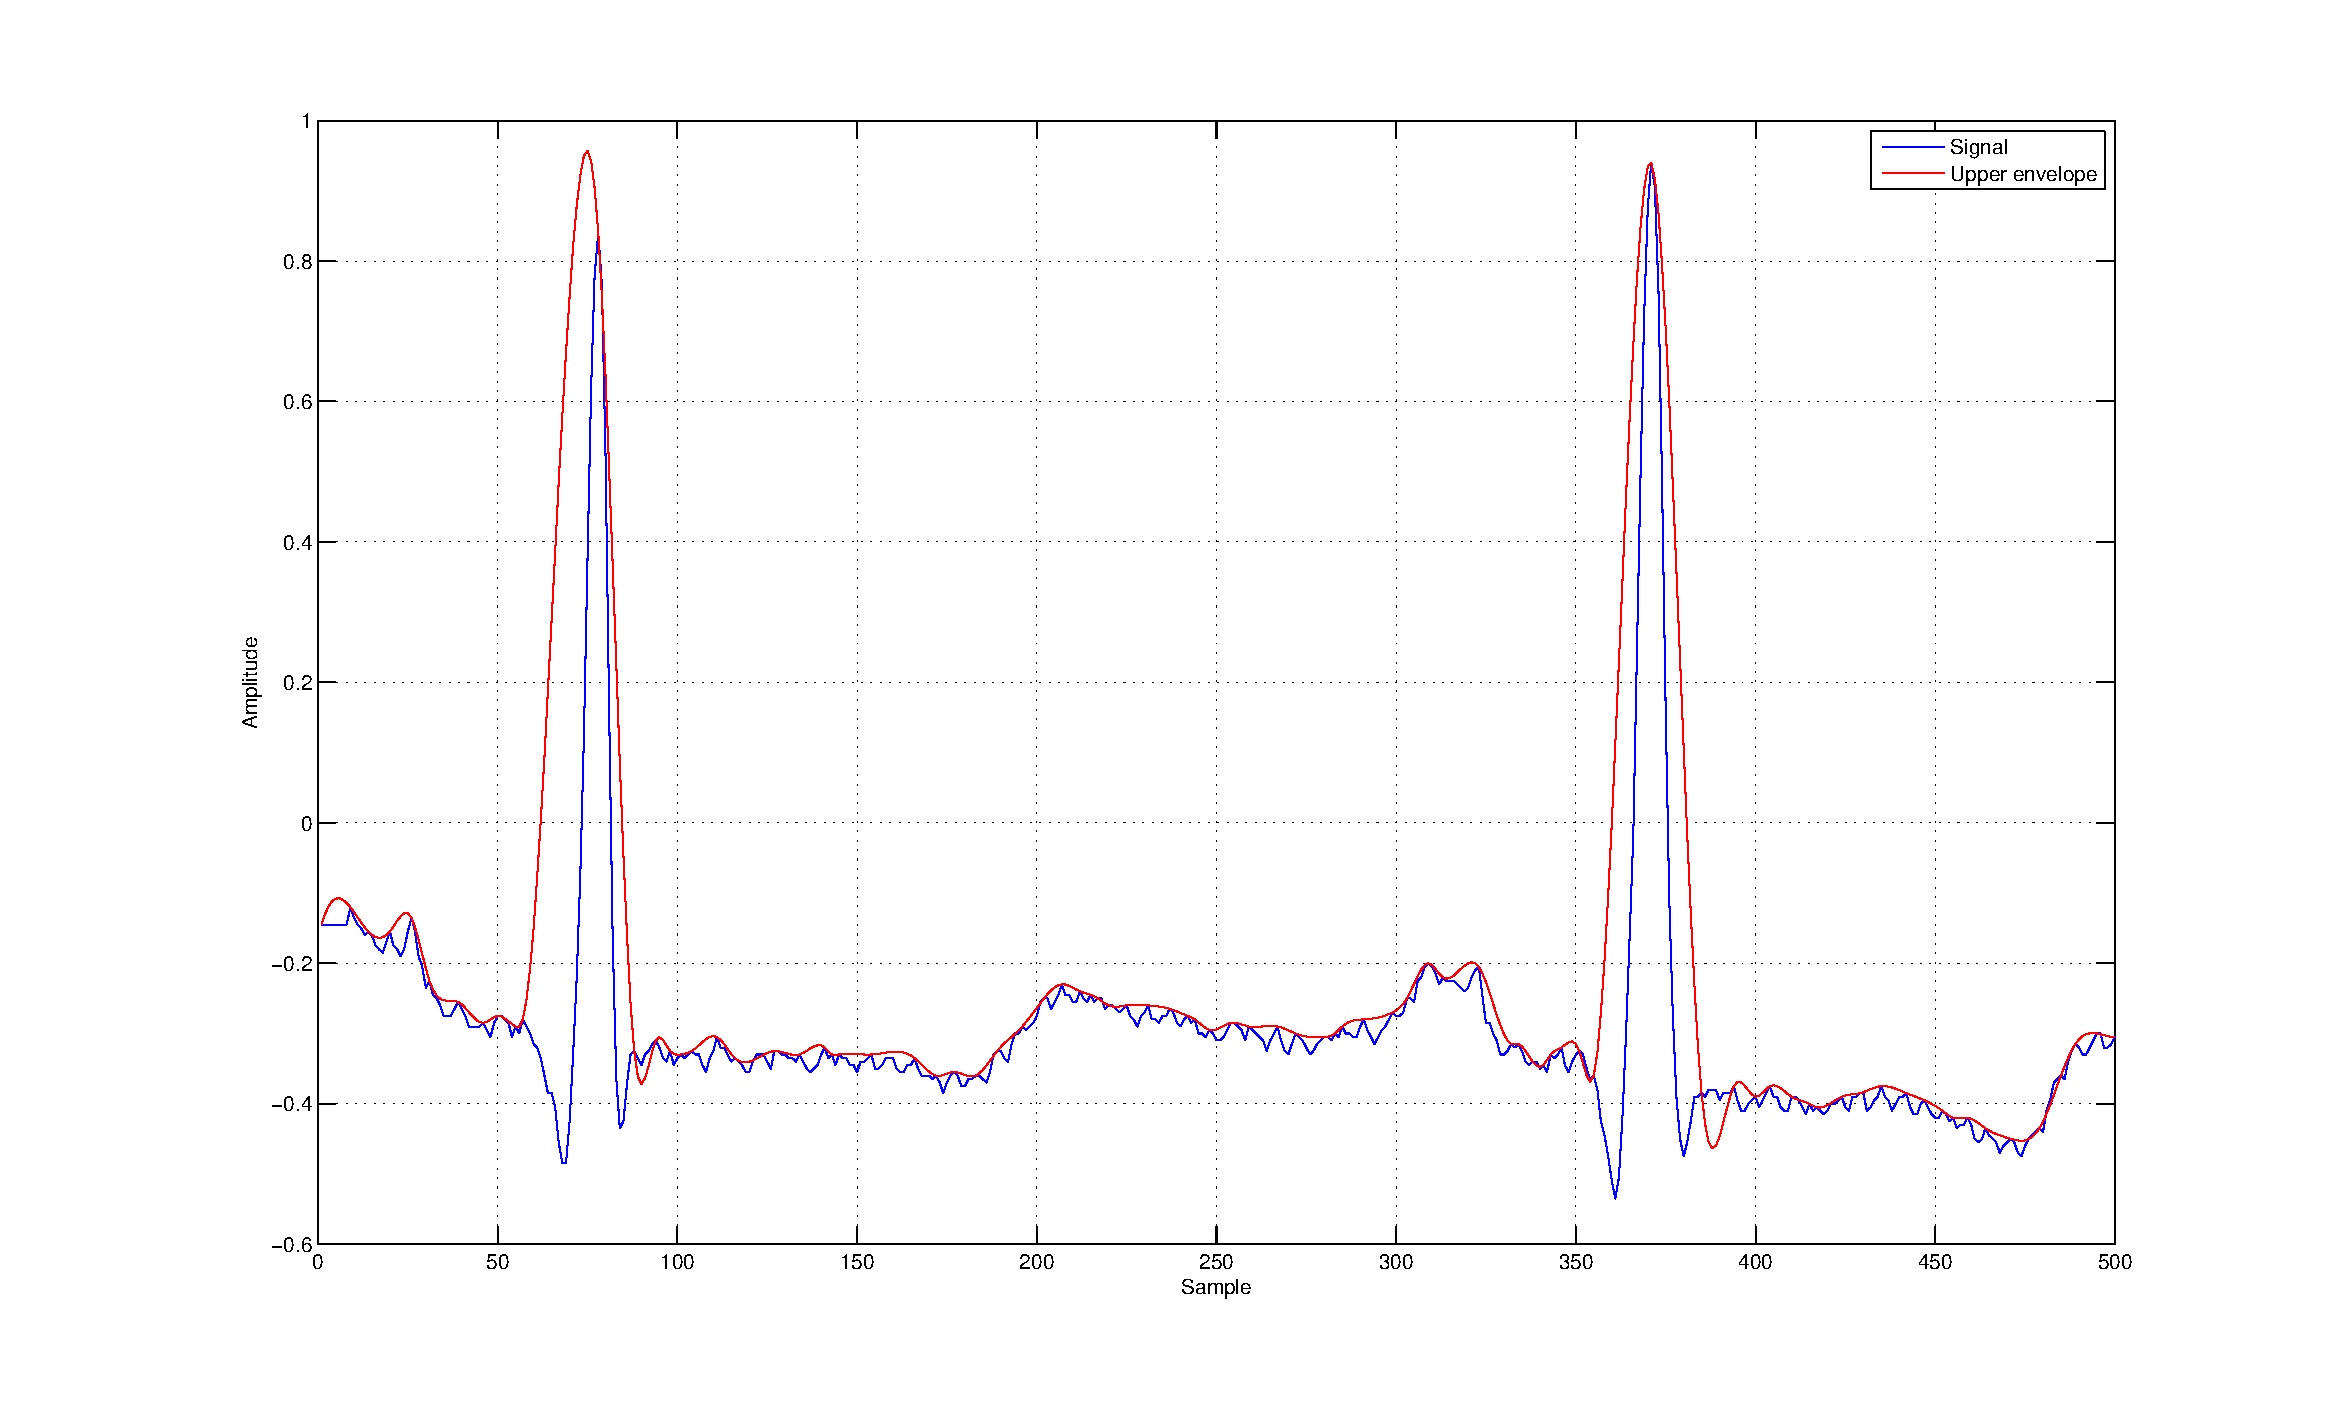
\includegraphics[width=\textwidth]{../img/upperenvelope.eps}
        \caption{Sygnał wraz z~górną obwiednią}
        \label{fig:upperenvelope}
    \end{figure}
    \newpage
    \item Znalezienie wszystkich lokalnych minimów i~połączenie ich za pomocą
    funkcji sklejanej, która tworzy dolną obwiednię sygnału
    (rys.~\ref{fig:lowerenvelope}).
    \begin{figure}[!ht]
        \centering
        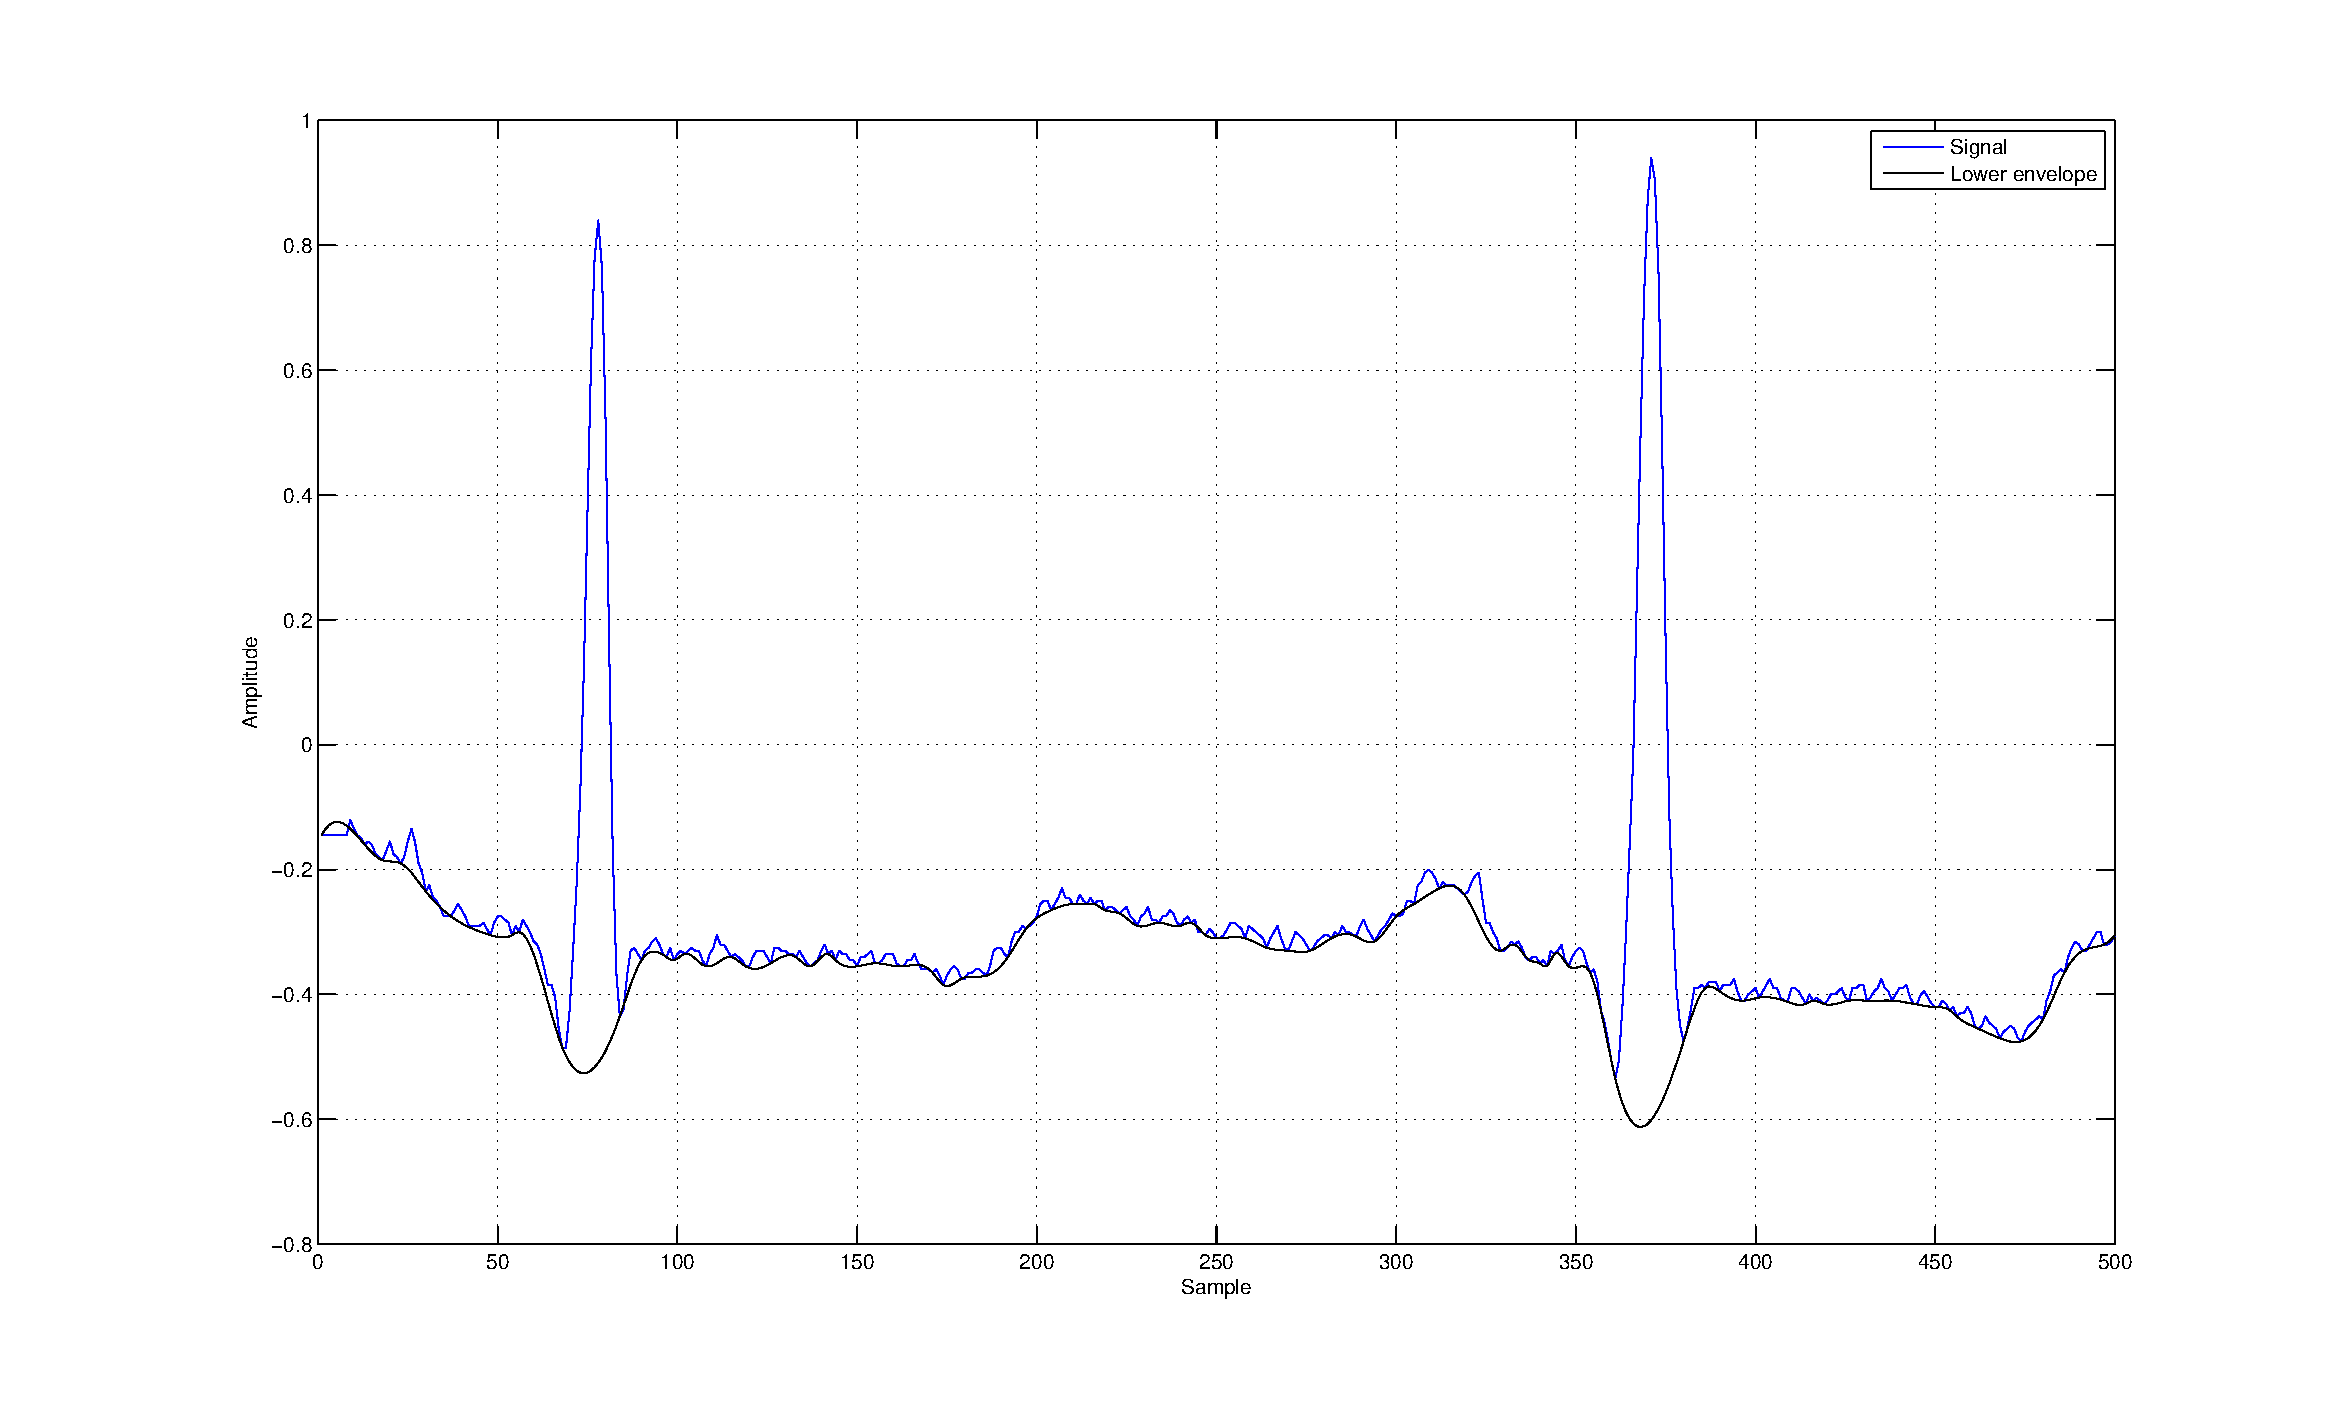
\includegraphics[width=\textwidth]{../img/lowerenvelope.eps}
        \caption{Sygnał wraz z~dolną obwiednią}
        \label{fig:lowerenvelope}
    \end{figure}
    \item Wyznaczenie średniej $m_1[n]$ z~górnej i~dolnej obwiedni sygnału
    (rys.~\ref{fig:envelopemean}).
    \begin{figure}[!ht]
        \centering
        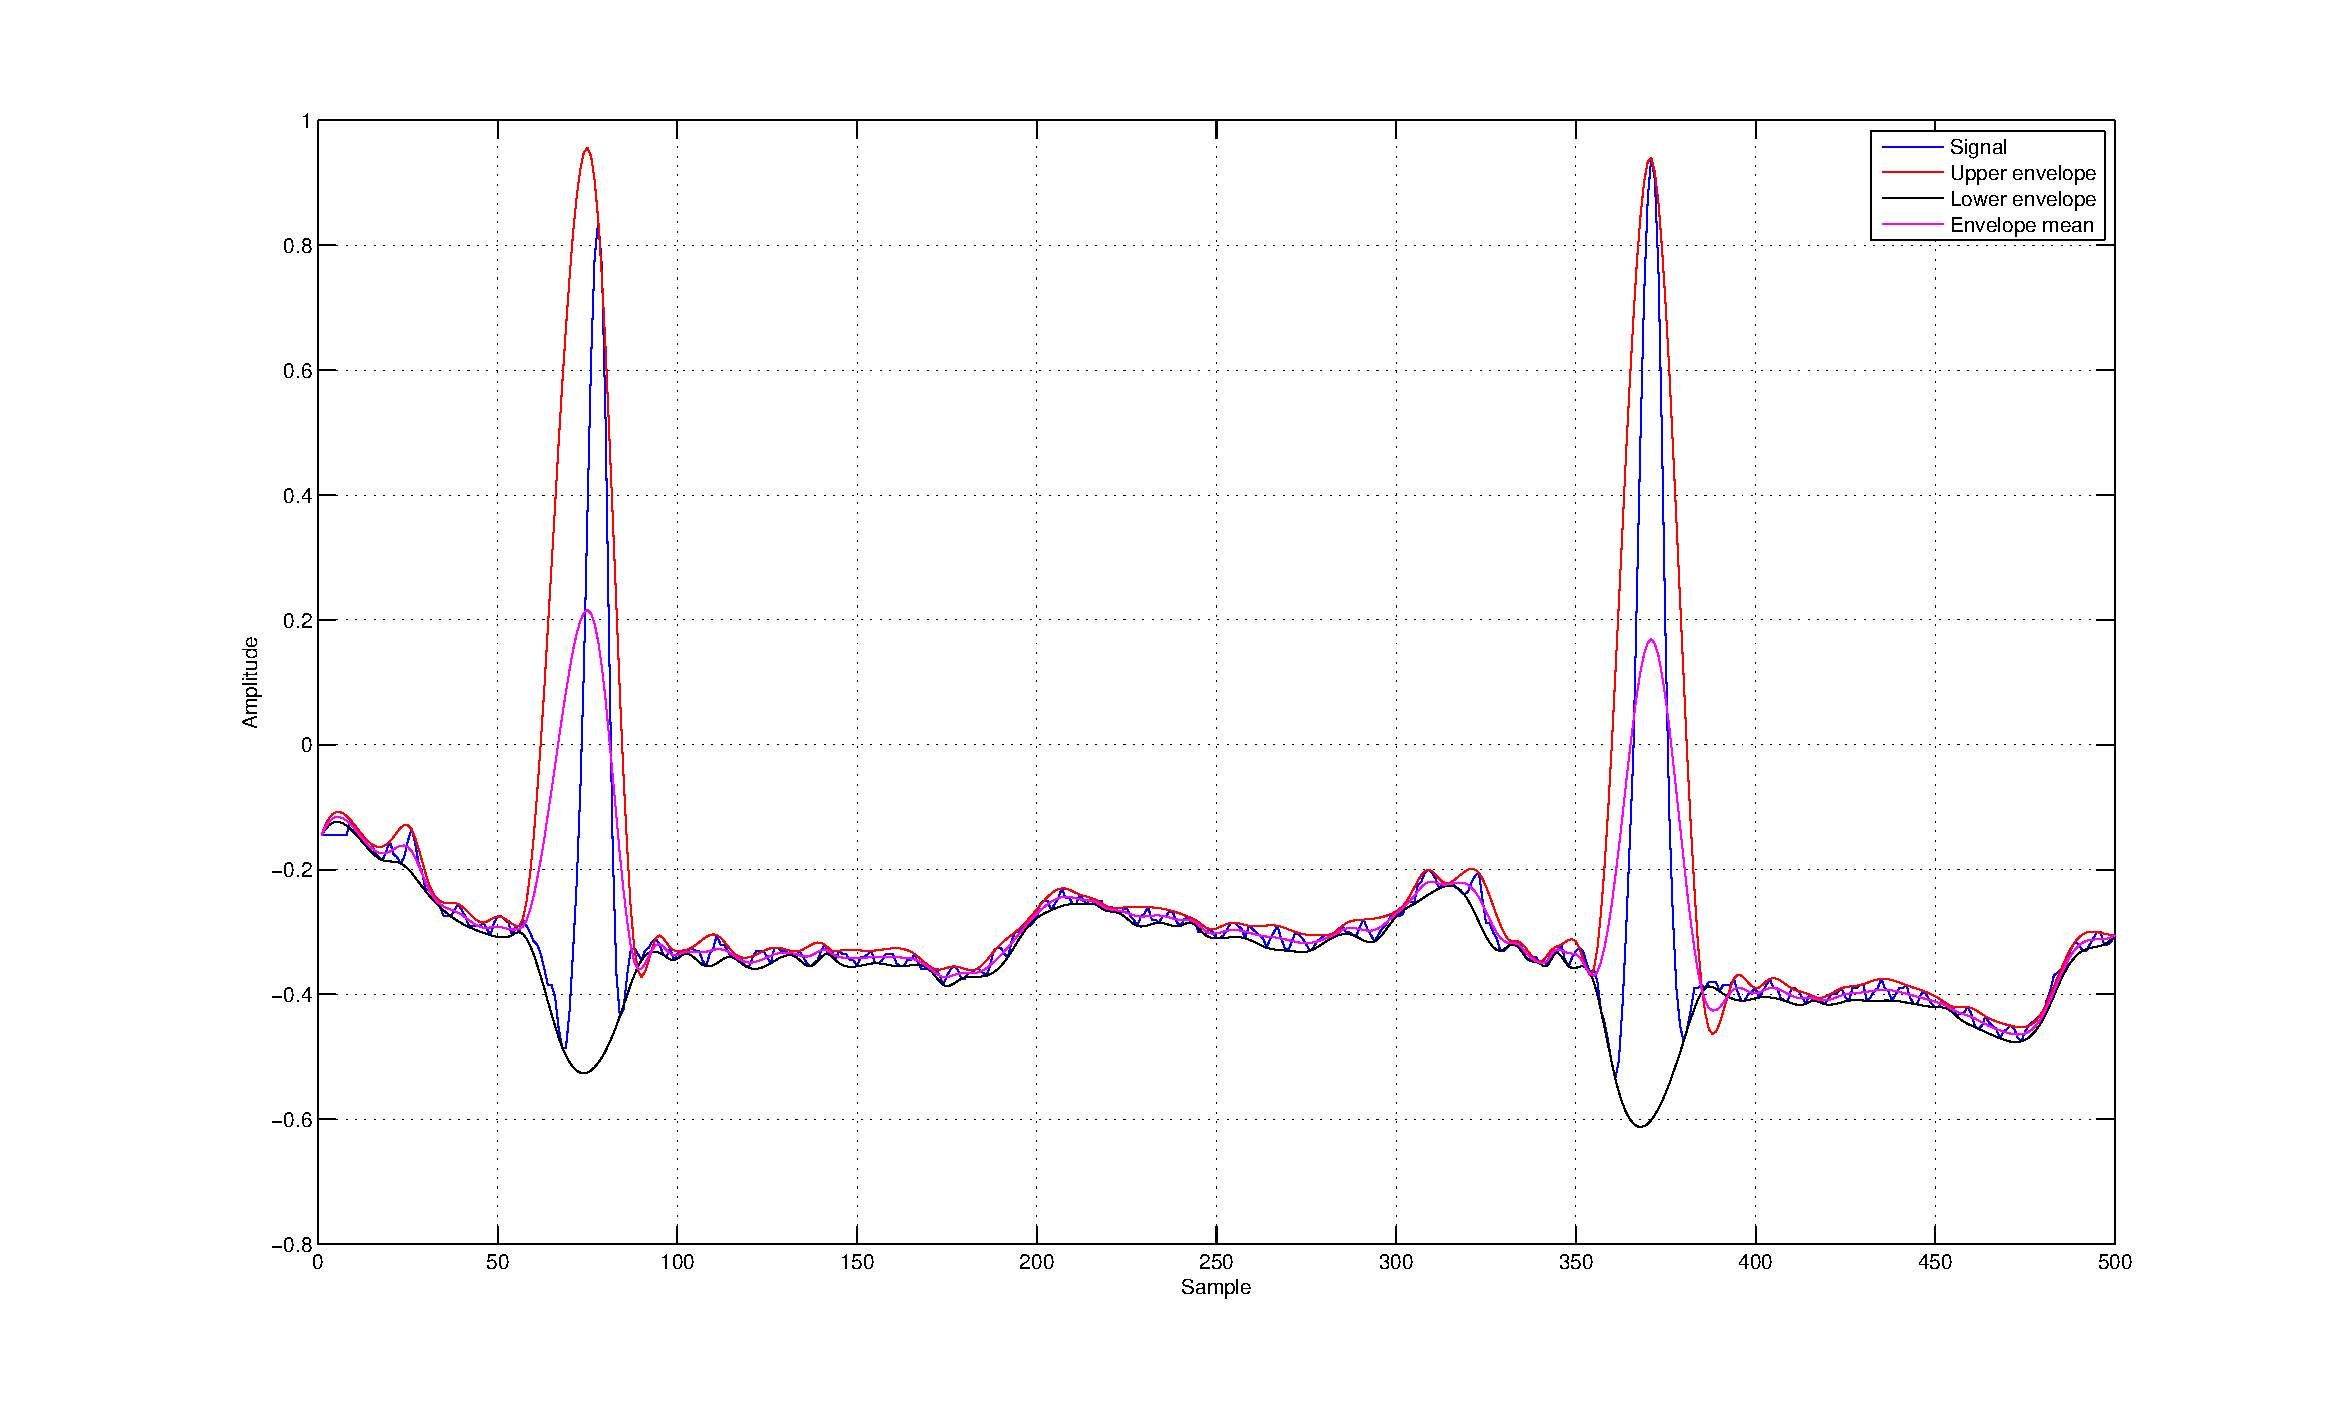
\includegraphics[width=\textwidth]{../img/envelopemean.eps}
        \caption{Sygnał wraz z~górną i~dolną obwiednią oraz ich średnią}
        \label{fig:envelopemean}
    \end{figure}
    \item Odjęcie od oryginalnego sygnału $x[n]$ średniej $m_1[n]$ w~celu
    otrzymania składowej $h_1[n]$ (rys.~\ref{fig:firstcomponent}).
    \begin{figure}[!ht]
        \centering
        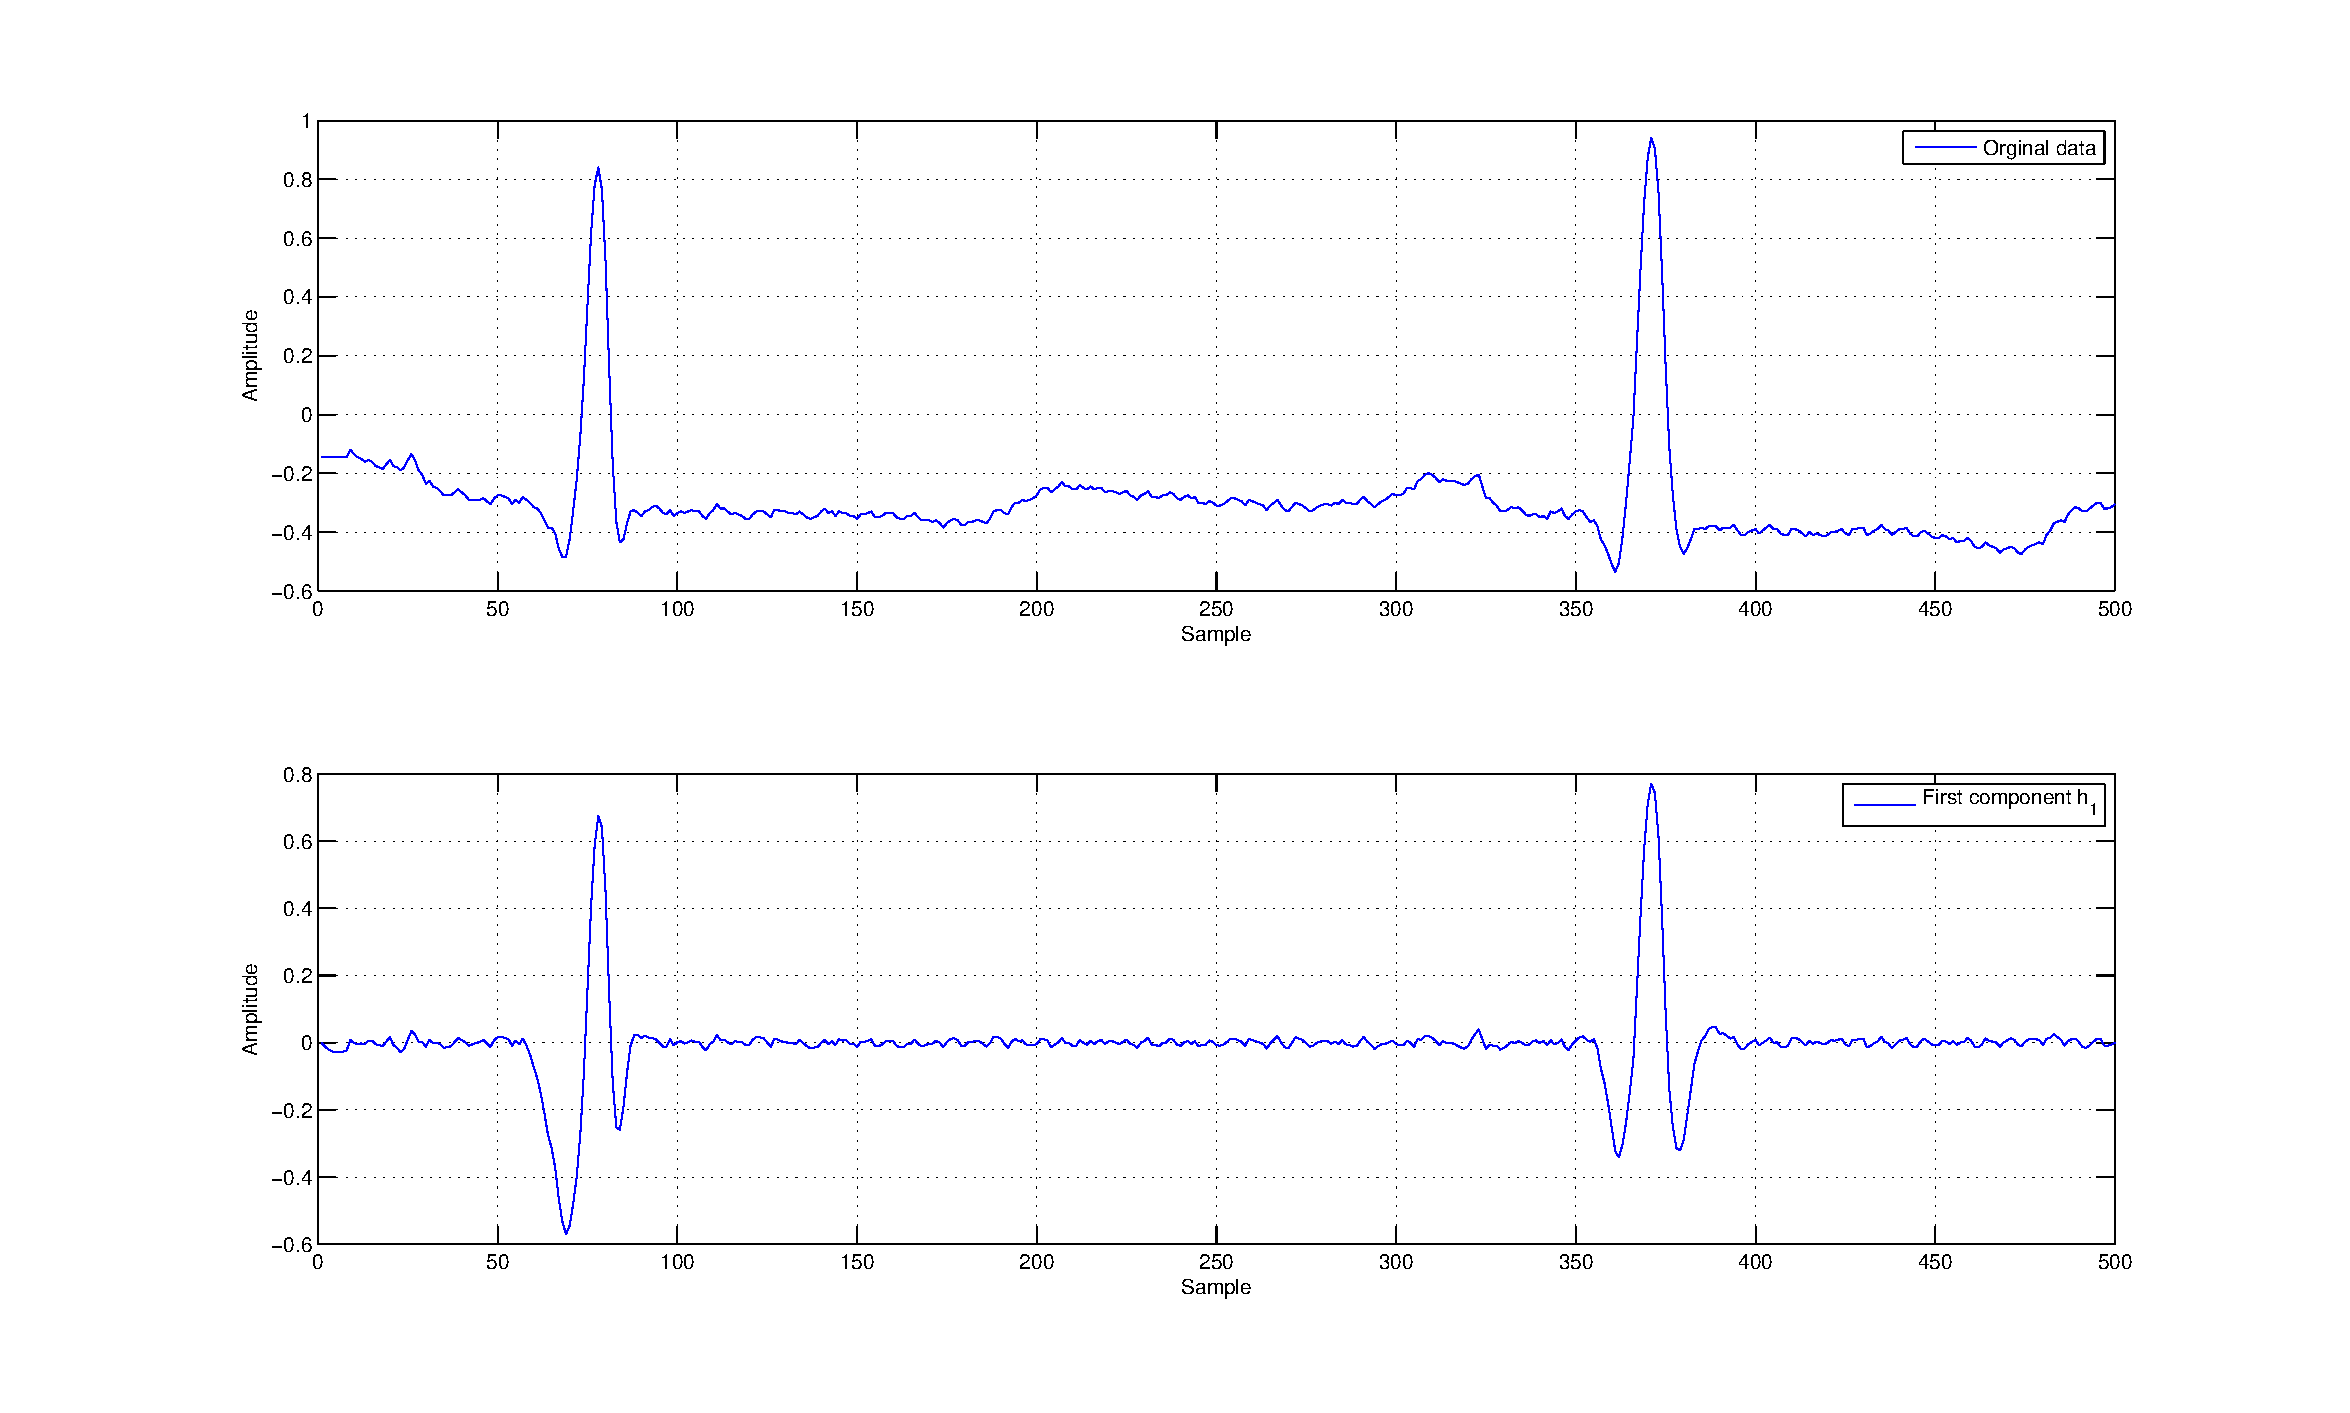
\includegraphics[width=\textwidth]{../img/firstcomponent.eps}
        \caption{Sygnał bazowy $x[n]$ oraz pierwsza składowa $h_1[n]$}
        \label{fig:firstcomponent}
    \end{figure}
    \item Podstawienie za $h_0[n]$ sygnału oryginalnego oraz sprawdzenie warunku
    stopu dla procesu ,,siftingu'':
    \begin{equation}
        SD = \sum\limits_{n = 0}^{N} \frac{\left| h_i[n] - h_{i - 1}[n]
        \right|^2}{h_{i - 1} ^ 2[n]}
    \end{equation}
    gdzie:
    \begin{itemize}
        \item $n$ --~numer próbki,
        \item $N$ --~liczba wszystkich próbek,
        \item $SD$ --~odchylenie standardowe sygnału.
    \end{itemize}
    \item Jeśli składowa $h_1[n]$ spełnia powyższy warunek stopu --~odchylenie
    standardowe mniejsze od przyjętego limitu --~$h_1[n]$ jest pierwszą składową
    IMF $c_1[n]$. Wyznaczenie reszty z~sygnału $r_1[n] = x[n] - h_1[n]$
    i~przyjęcie jej za nowy sygnał oryginalny oraz powrót do punktu 1.
    \item Jeśli warunek stopu nie jest spełniony, to przyjęcie $h_1[n]$ za nowy
    sygnał oryginalny oraz wykonanie na nim kolejnej operacji ,,siftingu''
    (powrót do punktu 1.).
\end{enumerate}

Po otrzymaniu $L$ sygnałów składowych, sygnał oryginalny $x[n]$ można
przedstawić przy pomocy sumy:
\begin{equation}
    x[n] = \sum\limits_{i = 1}^L c_i[n] + r_L[n]
\end{equation}

\newpage

Przykładowy sygnał ECG rozłożony na trzy składowe IMFs oraz resztę $r_3$
przedstawiony został na rysunku~\ref{fig:sampleimfs}.
\begin{figure}[!ht]
    \centering
    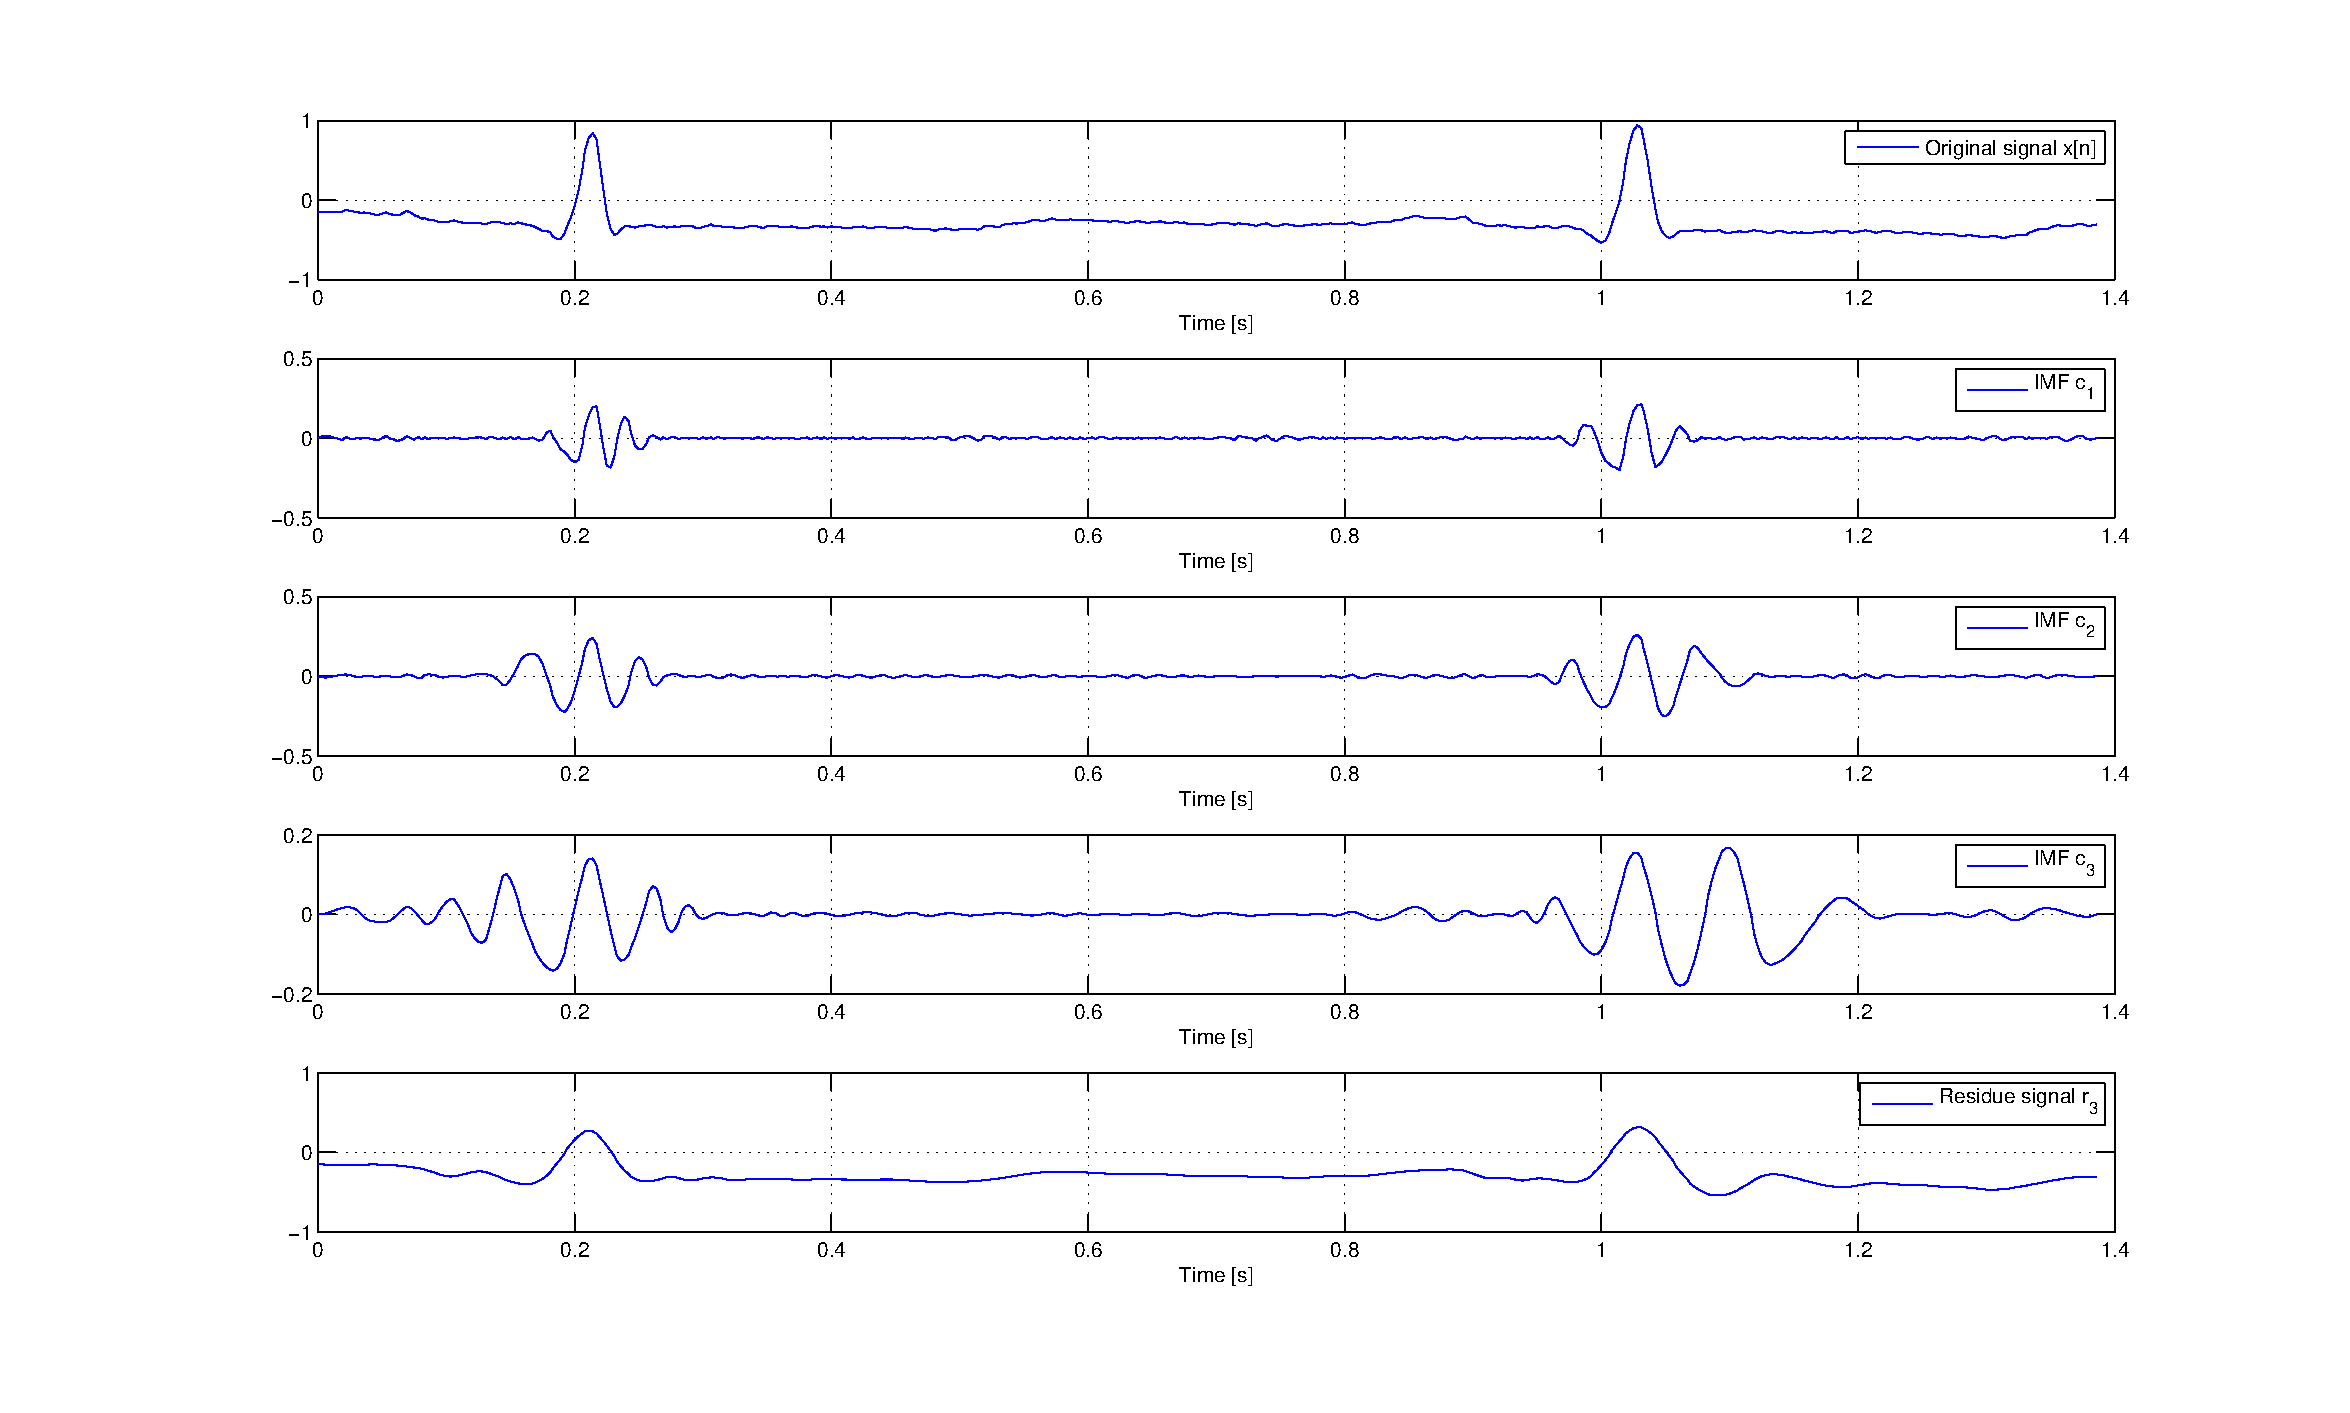
\includegraphics[width=\textwidth]{../img/sampleimfs.eps}
    \caption{Sygnał bazowy $x[n]$, trzy pierwsze składowe IMF-y oraz reszta
    $r_3$}
    \label{fig:sampleimfs}
\end{figure}

\newpage

\subsection{Odtwarzanie sygnału EKG}
\indent

W odtworzenia niezaszumionego sygnału EKG należy zsumować IMF-y niosące ze sobą
istotne informacje. Wybór odpowiednich IMF-ów jest istotnym czynnikiem
wpływającym na jakość filtracji. Odrzucenie zbyt wielu składowych spowoduje duże
zniekształcenie badanego sygnału. Odrzucenie zbyt małej liczby składowych
niedostatecznie odfiltruje szumy. Zazwyczaj początkowe składowe IMF zawierają
szum, im wyższy rząd składowej, tym więcej istotnej informacji niesie.

Na rysunku \ref{rys:example_ekg}, przedstawiono przykładowy sygnał EKG
odfiltrowany metodą EMD dla różnej liczby odrzuconych początkowych składowych
IMF.

\begin{figure}[!htb]
    \begin{center}
        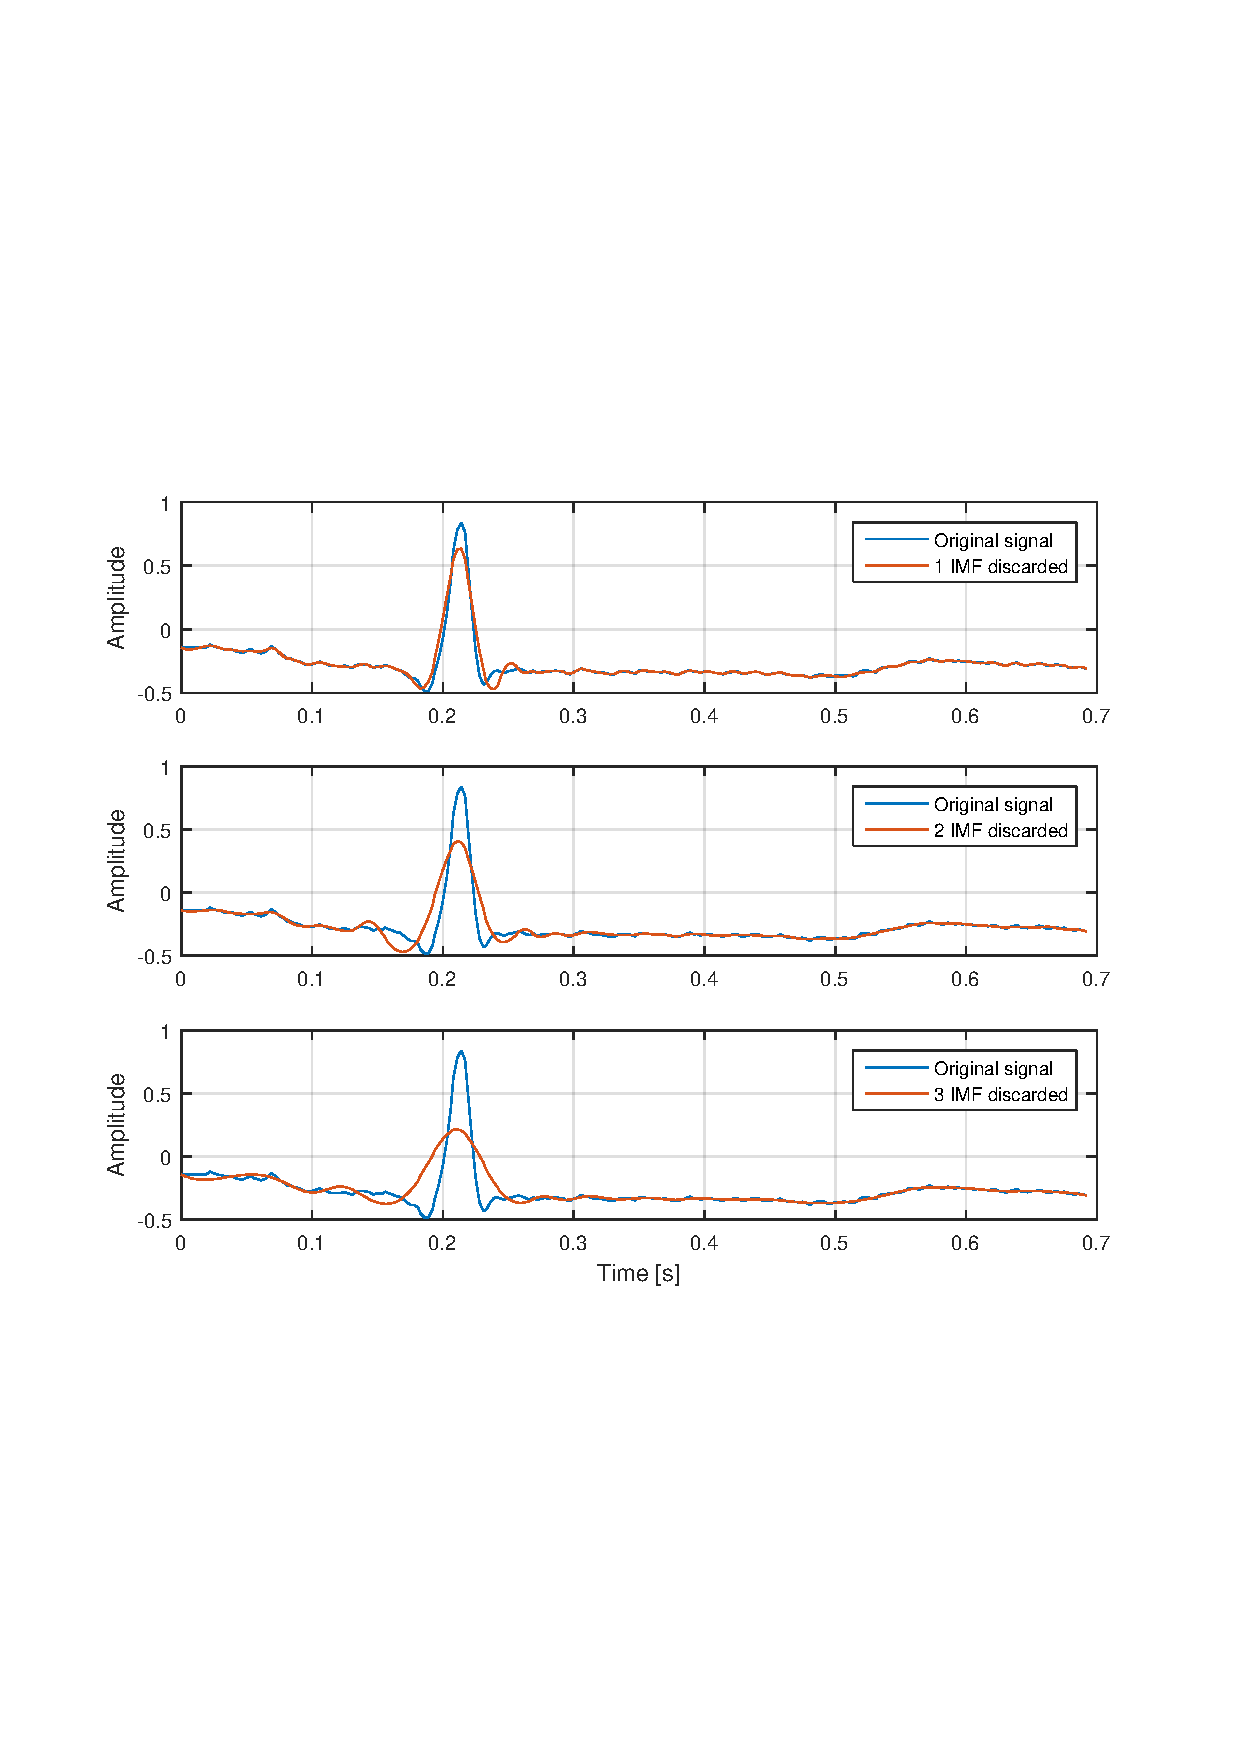
\includegraphics[width=14cm,trim=3cm 8cm 3cm 8cm,clip]
        {../img/ka_example.pdf}
    \end{center}
    \caption{Przykładowy przebieg EKG, na tle odfiltrowanych sygnałów o różnej
    liczbie odrzuconych składowych IMF}
    \label{rys:example_ekg}
\end{figure}


